% ===========================================================================
%  Results section for the SU pressure subset (products B/C/E/F of tab:dataSU).
%
%  Every figure below is produced by plot_report.py in THIS directory, which
%  reads only the framework upload products in ./data/SU/ -- the report
%  directory is self-contained: tex, figures, plotting code and the upload
%  data (the baseline figure reads the phase-1/phase-2 pipeline files, as it
%  is figure-only). The
%  quantitative numbers quoted in the text (rejection variance fractions,
%  baseline drift) are printed by the same script. The PNGs live alongside
%  this file, so compile from this directory or add
%      \graphicspath{{./}}
%  to the preamble so the local figures are found.
% ===========================================================================
\section{Experimental Results}\label{sec:results}

Every pressure signal is reported in two forms. The \emph{raw} product is the uncalibrated pressure in Pascals (microphone sensitivity and static-pressure compensation only); the \emph{production} product additionally applies the measured pinhole-to-nose-cone and nose-cone-to-reference transfer functions, mean removal, and a Wiener facility-noise rejection; no digital band filtering is applied to the signals -- the analog anti-alias low-pass acts upstream in hardware, and the reported band is enforced simply as a mask on the computed spectra. The Wiener filter is trained on the smooth-wall baseline and is constructed to remove \emph{facility} (background acoustic) noise only. It deliberately does not target the dipole and quadrupole sources generated in the freestream by a protrusion or bump; although these originate away from the wall they leave an imprint on the wall pressure and are properly part of the signal. Concretely, the rejection is \emph{not} an adaptive cancellation referenced to the freestream microphone of the case being processed: the Wiener rejection transfer function (a FIR kernel identifying the facility-to-wall acoustic path) is computed once on the smooth-wall baseline, where the freestream reference carries facility noise only, and is applied unchanged to the protrusion cases, where it filters the simultaneously recorded nose-cone signal to form the facility-noise estimate that is subtracted. Raw and production spectra are shown together throughout so that the effect of the rejection is visible.

The production wall-pressure spectra are presented premultiplied and inner-scaled: the abscissa is the viscous time scale $T^+ = u_\tau^2/(\nu f)$ (so large $T^+$ corresponds to low frequency) and the ordinate is ${f\phi_{pp}}^{+} = f\phi_{pp}/\tau_w^2 = f\phi_{pp}/(\rho^2 u_\tau^4)$, the premultiplied wall-pressure spectrum normalised by the wall shear stress $\tau_w = \rho u_\tau^2$, formed with the measured per-station friction velocity. The raw wall-pressure and freestream spectra are \emph{not} inner-scaled -- the raw signal is uncalibrated and the freestream reference is not a wall quantity, so inner scaling would not be meaningful -- and are instead shown as the dimensional PSD $\phi_{pp}$ [Pa$^2$/Hz] against frequency $f$ [Hz] on log--log axes, without premultiplication (premultiplied forms are reserved for the semi-logarithmic inner-scaled presentation, where equal areas correspond to equal energy). The three production Reynolds numbers are set by tunnel pressurisation to $0$, $50$ and $100$~psig, spanning $Re_\tau^{\mathrm{smooth}} \approx 1.3\times10^{3}$, $5.3\times10^{3}$ and $9.1\times10^{3}$ at the smooth-wall reference conditions; each wall-pressure figure is therefore laid out as three panels, one per pressurisation (labelled by $Re_\tau^{\mathrm{smooth}}$), and every panel reports all four pinhole stations P1--P4, ordered in the legends by their streamwise position $x$. Because the pinhole diameter is fixed ($d = 70~\mu\mathrm{m}$), the viscous-scaled resolution $d^{+} = d\,u_\tau/\nu$ grows with Reynolds number from $d^{+}\approx 2.5$ at $0$~psig to $d^{+}\approx 18$ at $100$~psig, approaching the $d^{+}\approx 20$ threshold beyond which high-frequency attenuation of the wall-pressure spectrum becomes significant.

The reported wall-pressure band is limited above by a per-station cut
\begin{equation*}
  f_{\mathrm{cut}} \;=\; \min\!\left(f_{H},\; \frac{u_\tau^2}{\nu\,T^+_{\mathrm{cut}}}\right),
\end{equation*}
the smaller of a Helmholtz-resonance guard and a spatial-resolution limit. The pinhole cavity resonates at ${\approx}1.4$~kHz; the resonance frequency is set by the cavity geometry and the speed of sound, so it is the \emph{same} at every pressurisation (only its damping falls as the density rises), and it must be excluded by a fixed guard $f_{H} = 1.2$~kHz rather than by a cut that scales with $Re_\tau$. The semi-anechoic calibration cannot reliably invert the high-$Q$, mounting-sensitive resonance, so the band is terminated below it rather than corrected through it. The second term, $T^+ \ge T^+_{\mathrm{cut}} = 10$ evaluated with the measured per-station $u_\tau$, excludes viscous time scales too fine for the pinhole to resolve as $d^+$ grows; at the smooth-wall reference conditions it corresponds to $1.9$, $8.0$ and $13.1$~kHz and never binds, so the resonance guard sets $f_{\mathrm{cut}} = 1.2$~kHz at every condition. Only at the lowest-$u_\tau$ fence stations at $0$~psig does the resolution term bind instead, slightly below the guard (${\approx}0.95$--$1.15$~kHz). In viscous units the reported band therefore shortens as $Re_\tau$ grows: the smallest reported time scale is $T^+ \approx 16$, $66$ and $109$ at $0$, $50$ and $100$~psig. The cut is applied simply as a mask on the computed spectra -- no time-domain filtering is involved -- and the per-station value travels with each dataset as \texttt{f\_cut\_Hz}; it sits well below the per-condition analog anti-alias low-pass (\texttt{analog\_LP\_filter\_Hz} $= 2100$, $4700$, $14\,100$~Hz). The nose-cone freestream microphone is not pinhole-mounted and is not subject to the cut.

\subsection{Case B1: 2-$\delta$ protrusions}
\subsubsection{Shear stress}

\subsubsection{Freestream pressure}

\begin{figure}
    \centering
    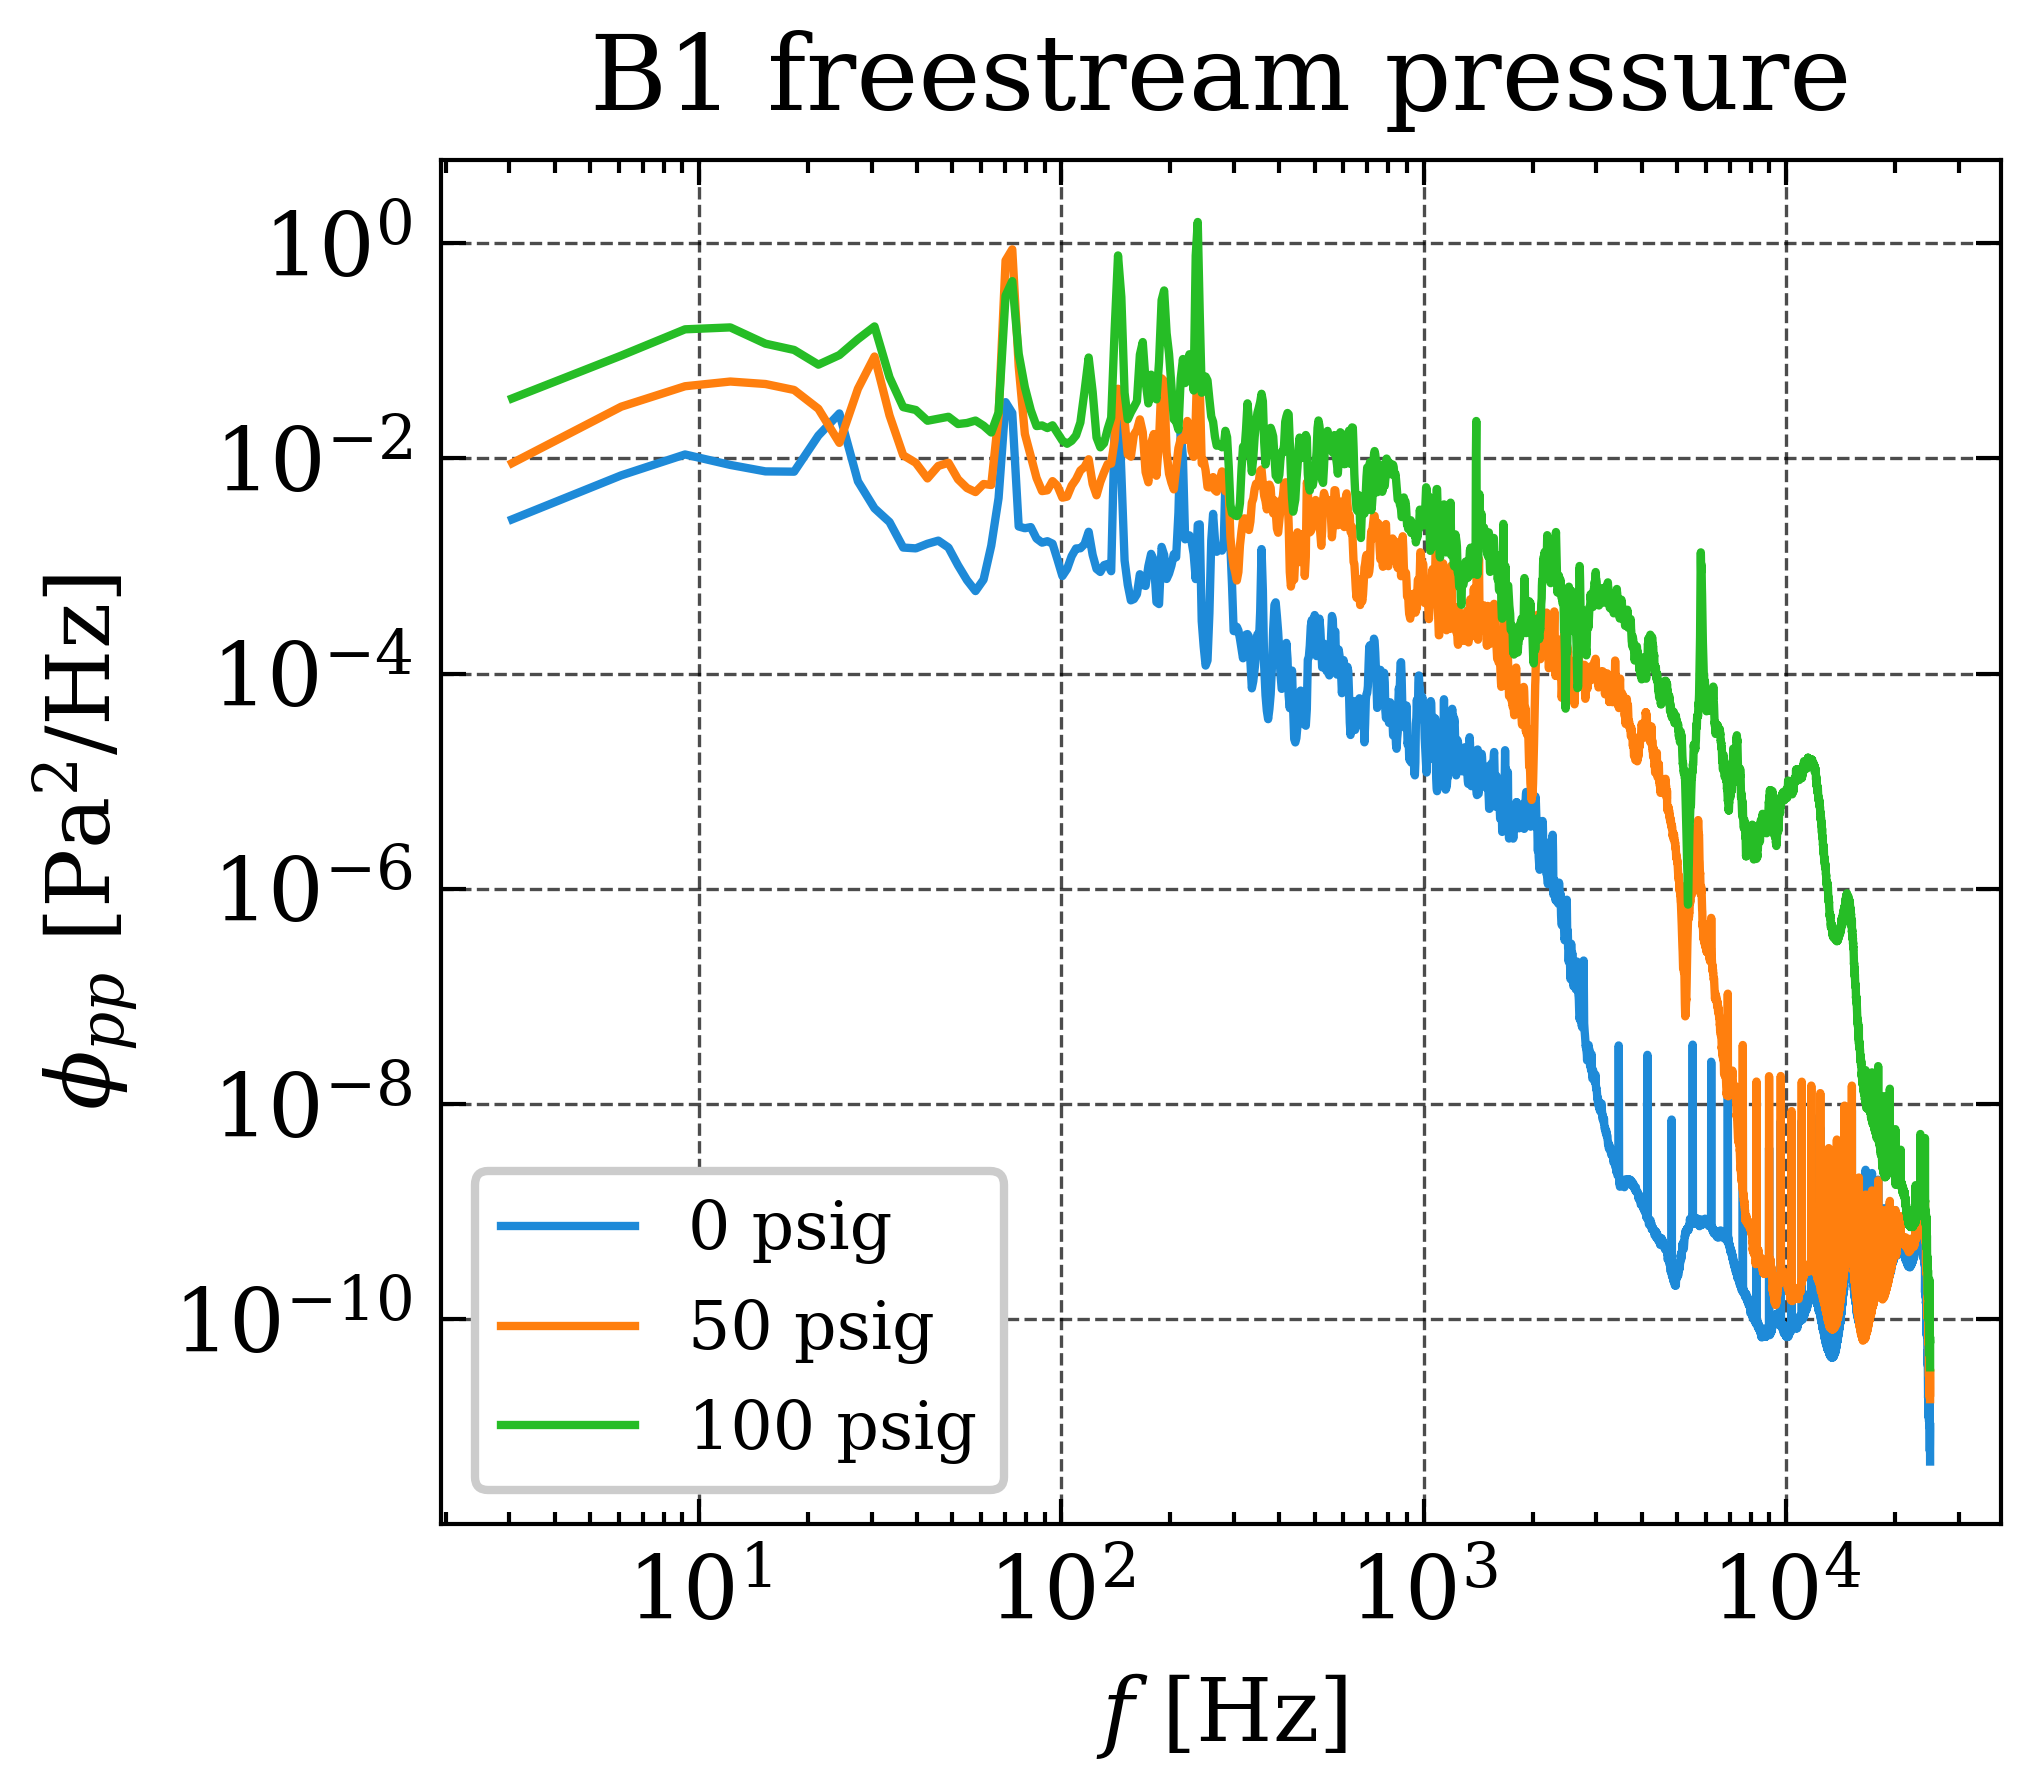
\includegraphics[width=0.6\linewidth]{B1_freestream}
    \caption{Freestream pressure PSD recorded by the nose-cone microphone, $\phi_{pp}$ [Pa$^2$/Hz] against frequency, at the three pressurisations (SU HPWT). Data: \texttt{C\_B1\_freestreamp\_SU\_production.hdf5}.}
    \label{fig:fs pressure fence}
\end{figure}

Figure~\ref{fig:fs pressure fence} shows the freestream pressure recorded by the nose-cone microphone: broadband facility noise punctuated by discrete tunnel tones, its level rising steadily with pressurisation as the facility drive and dynamic pressure increase across the $0$--$100$~psig sweep. This signal is \emph{not} the reference that defines the wall-pressure noise rejection. On a protrusion case the nose-cone microphone hears the fence's own dipole and quadrupole radiation in addition to facility noise, so an adaptive Wiener filter referenced to it would remove genuine flow-generated wall-pressure content. Instead, the fixed rejection kernel identified on the smooth-wall baseline filters this simultaneously recorded signal to form the facility-noise estimate: what can be rejected is set by the smooth-wall-identified facility-to-wall transfer function, not by the spectral content of this case's freestream signal. The recording is reported both because it is the input the fixed kernel acts on and as the in-situ measurement of the freestream (facility plus protrusion-radiated) pressure environment.

\subsubsection{Wall pressure}

\begin{figure}
    \centering
    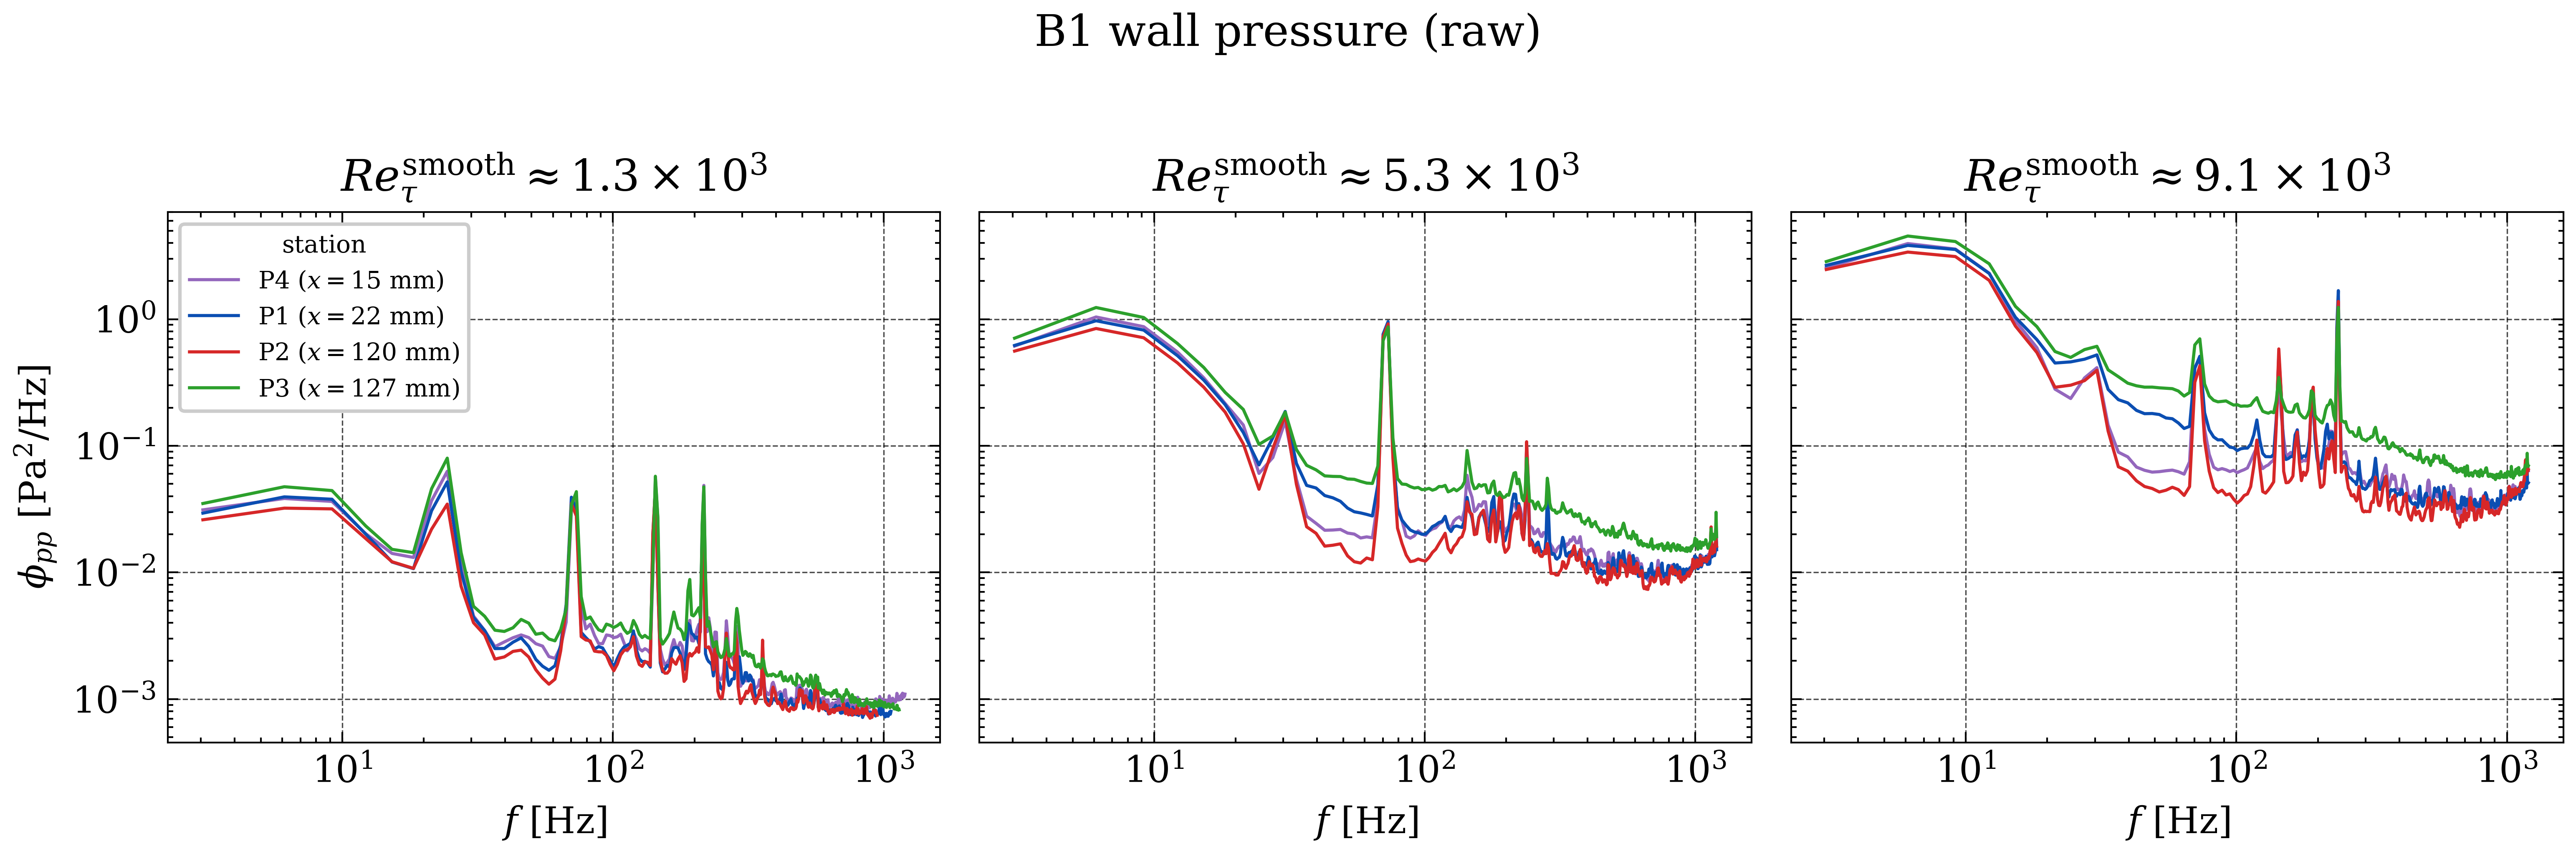
\includegraphics[width=\linewidth]{B1_wallp_raw}
    \caption{Raw wall-pressure PSD, $\phi_{pp}$ [Pa$^2$/Hz] against frequency, before facility-noise rejection (SU HPWT). One panel per pressurisation, labelled by $Re_\tau^{\mathrm{smooth}}$; each panel shows all four pinhole stations, ordered by streamwise position $x$. Every curve is terminated at its per-station reported-band edge $f_{\mathrm{cut}} = \min(f_H,\,u_\tau^2/(\nu T^+_{\mathrm{cut}}))\le 1.2$~kHz, below the ${\approx}1.4$~kHz pinhole Helmholtz resonance. Data: \texttt{B\_B1\_wallp\_SU\_raw.hdf5}.}
    \label{fig:wall pressure fence}
\end{figure}

Figure~\ref{fig:wall pressure fence} shows the wall-pressure spectra at the four stations with no facility-noise rejection applied, band-limited to the reported band. The discrete facility tones (${\approx}23$, $70$, $140$ and $230$~Hz) ride on top of the turbulent spectra at every station, and the overall levels rise with pressurisation as the dynamic pressure grows.

\begin{figure}
    \centering
    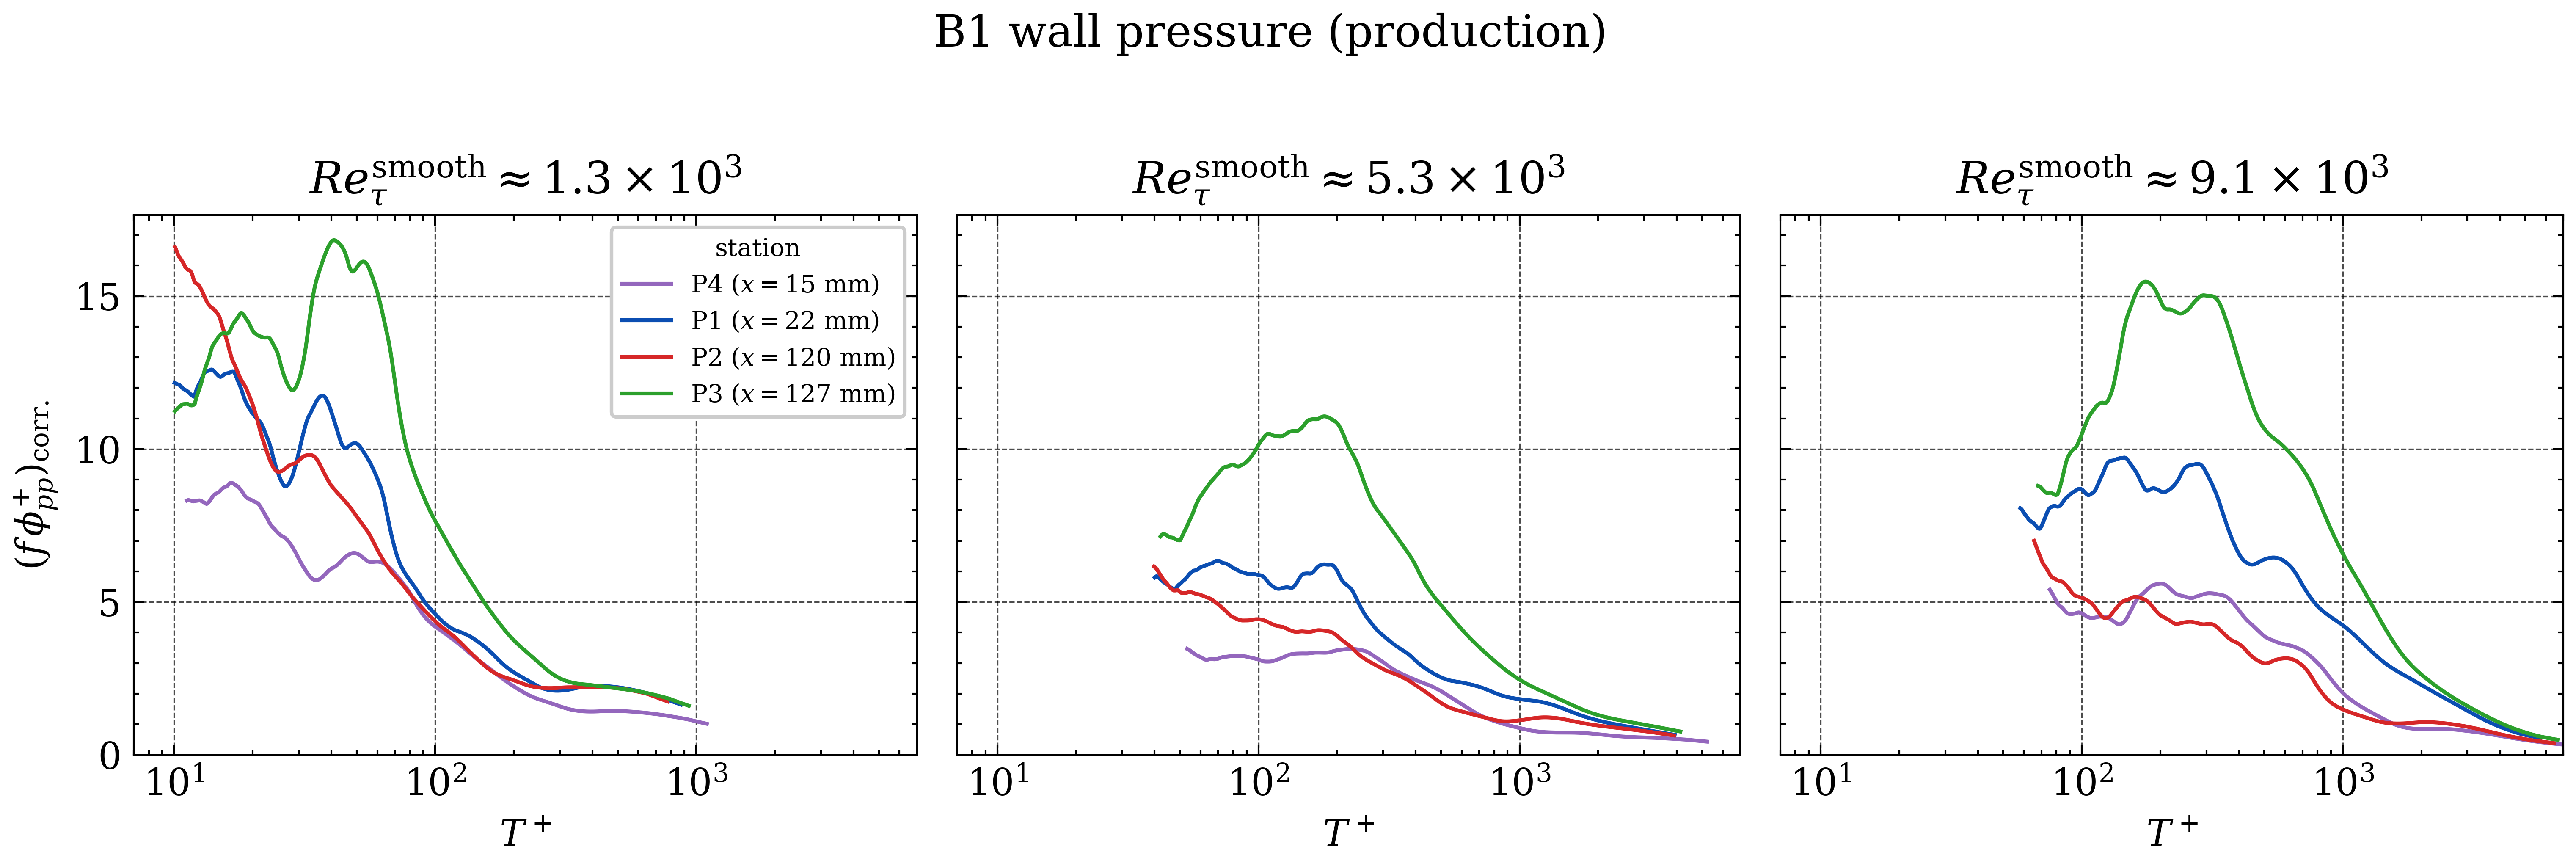
\includegraphics[width=\linewidth]{B1_wallp_production}
    \caption{Production (facility-noise-rejected via the smooth-wall-trained Wiener kernel), premultiplied, inner-scaled wall-pressure spectra (SU HPWT). One panel per pressurisation, labelled by $Re_\tau^{\mathrm{smooth}}$; all four stations per panel, each inner-scaled with its own measured $u_\tau$. The band edge $f_{\mathrm{cut}}$ sets the lowest $T^{+}$ shown for each curve. Data: \texttt{B\_B1\_wallp\_SU\_production.hdf5}.}
    \label{fig:wallp production fence}
\end{figure}

Figure~\ref{fig:wallp production fence} shows the same wall pressure after the smooth-wall-trained Wiener rejection, driven by the fence campaign's simultaneous nose-cone recording; comparing raw and production isolates the removed facility contribution. The transplant of the smooth-wall kernel is effective here because the facility-to-wall path is essentially unchanged by the fence: at the facility tones the measured nose-cone-to-wall transfer function of the fence records matches the smooth-wall one to within a few percent, with tone coherences of $0.8$--$0.96$. The rejection removes $41$--$50\%$ of the reported-band wall-pressure variance at $0$~psig (${\approx}60\%$ below $100$~Hz), $17$--$38\%$ at $50$~psig ($43$--$59\%$ below $100$~Hz) and $10$--$35\%$ at $100$~psig, and suppresses the facility tones to roughly a tenth of their un-rejected power. The rejected spectra retain a strong station-to-station variation -- levels several times the smooth-wall baseline, largest at P3 -- reflecting the different states of the fence-perturbed boundary layer at the four positions; this content is coherent flow signal that the smooth-wall-trained kernel deliberately leaves in place.

\subsection{Case B2: ``Eaton bump''}
\subsubsection{Shear stress}

\subsubsection{Freestream pressure}

\begin{figure}
    \centering
    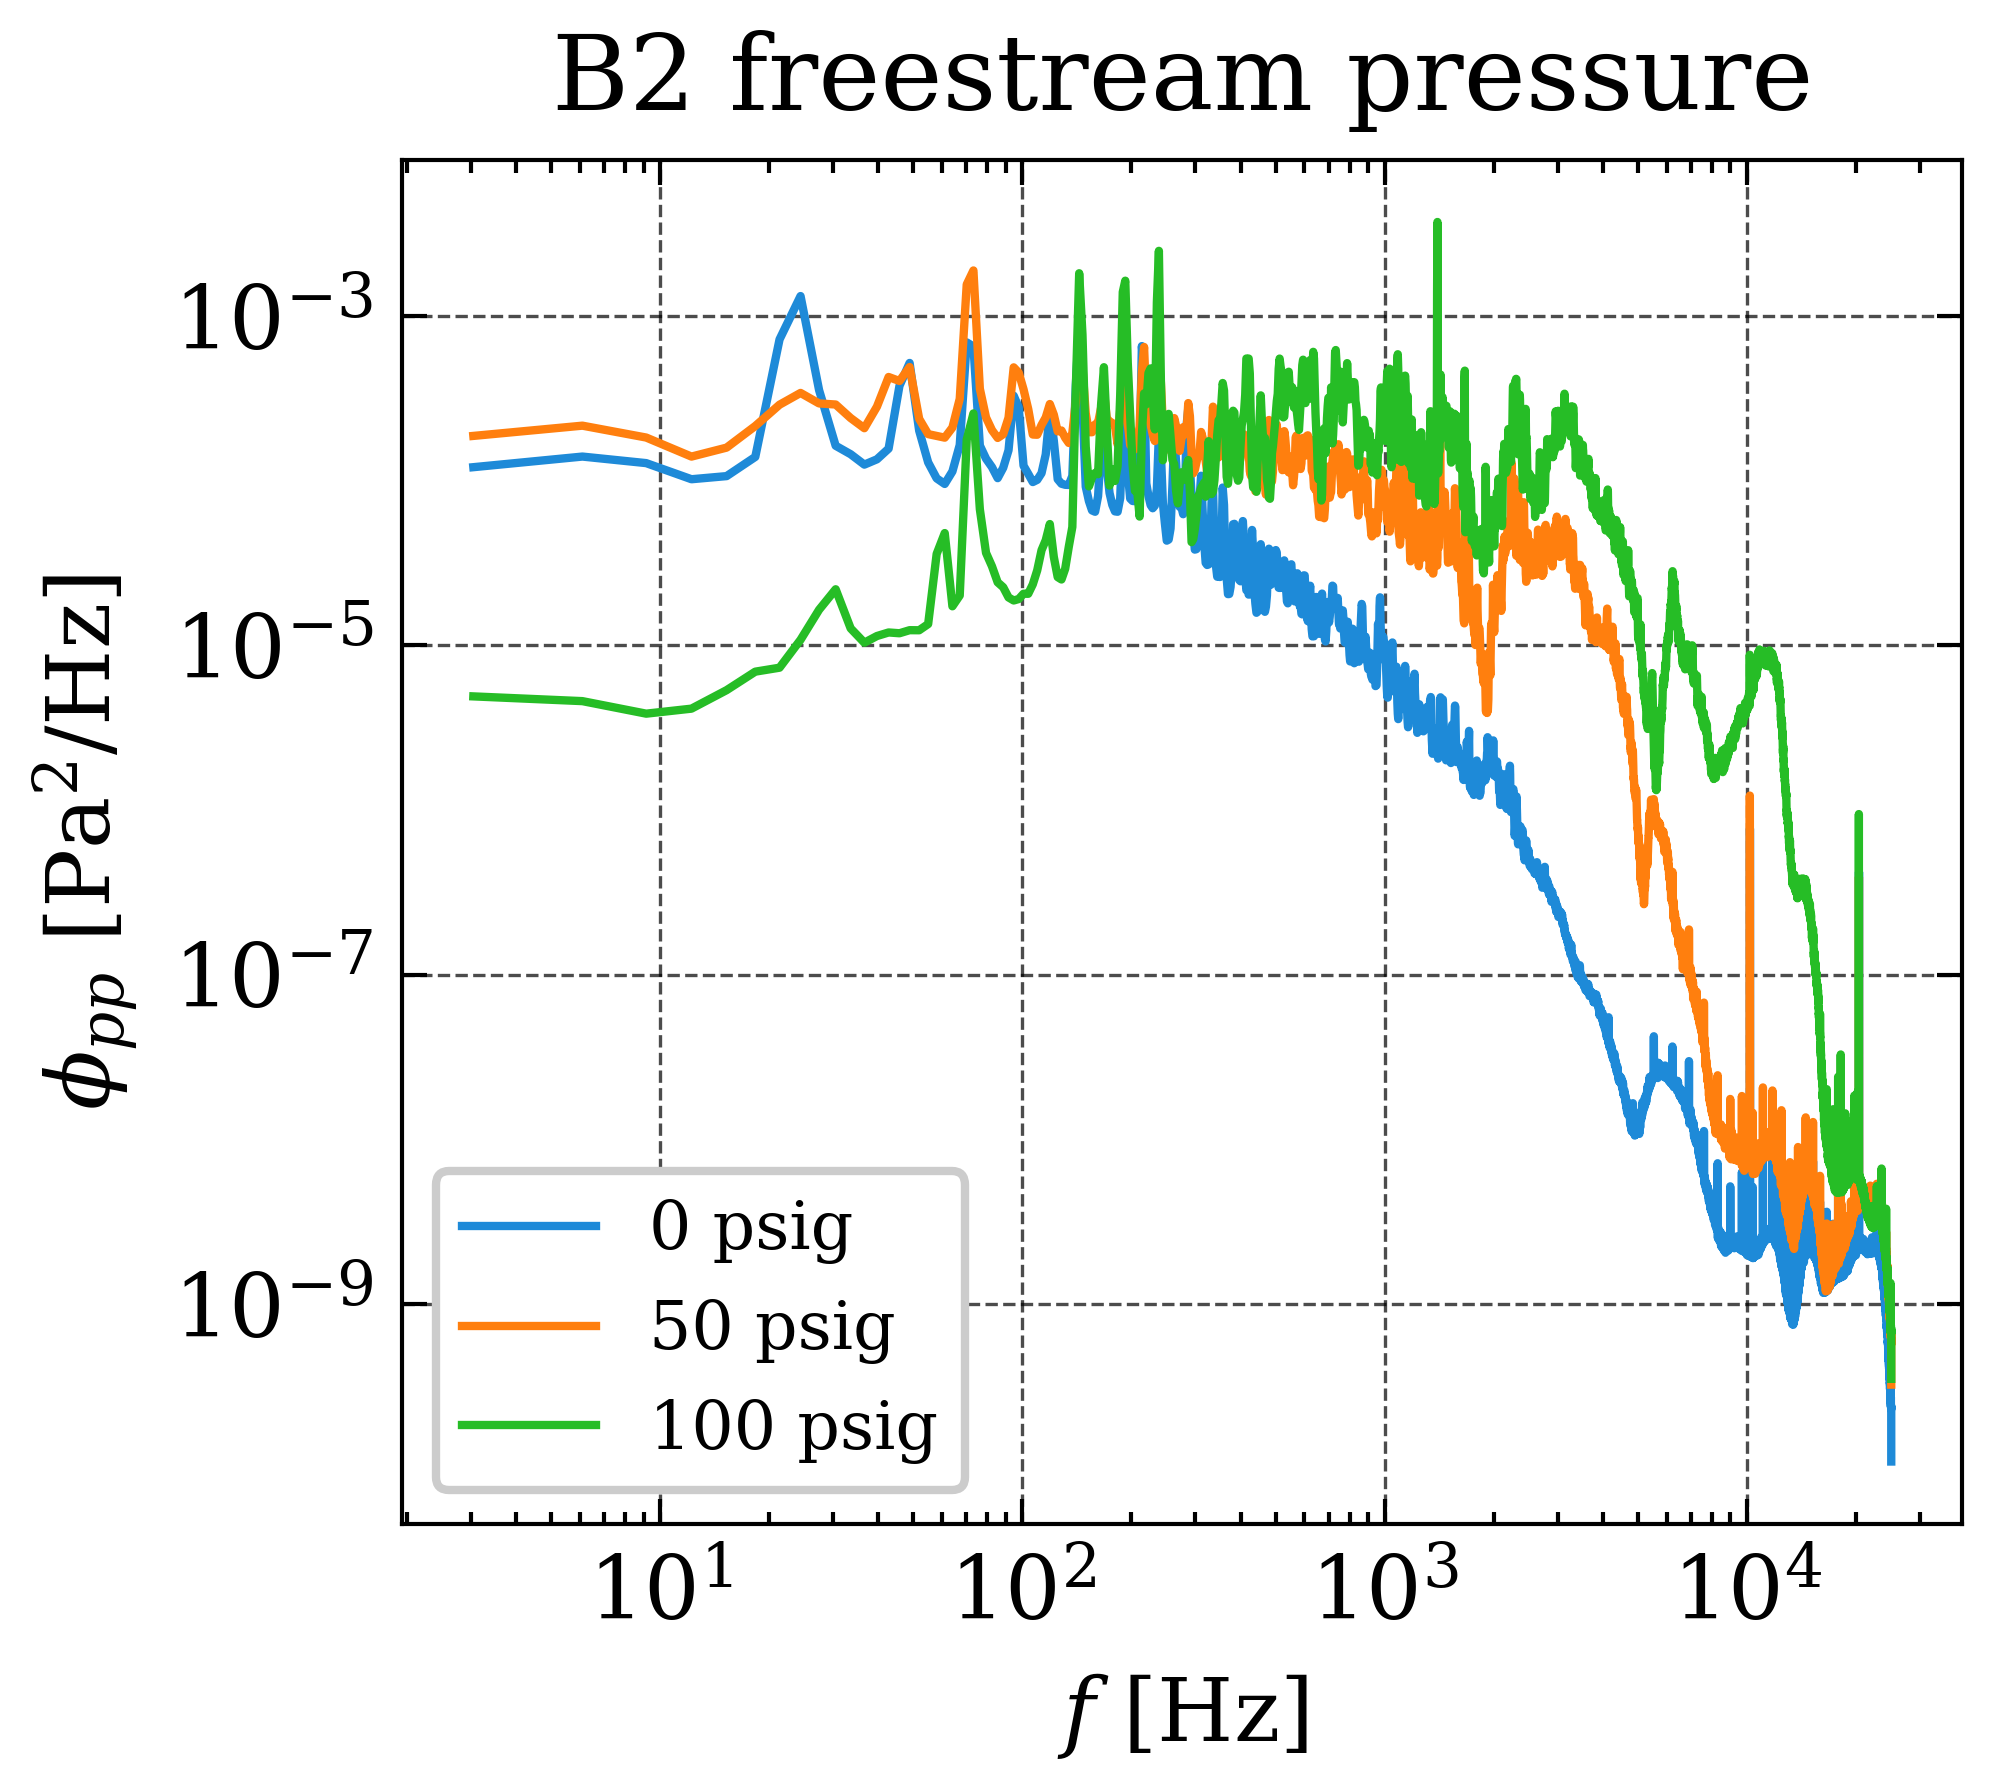
\includegraphics[width=0.6\linewidth]{B2_freestream}
    \caption{Freestream pressure PSD recorded by the nose-cone microphone, $\phi_{pp}$ [Pa$^2$/Hz] against frequency, at the three pressurisations (SU HPWT). Data: \texttt{F\_B2\_freestreamp\_SU\_production.hdf5}.}
    \label{fig:fs pressure bump}
\end{figure}

Figure~\ref{fig:fs pressure bump} shows the freestream pressure for the bump configuration. As for the fence, it is the input filtered by the fixed smooth-wall rejection kernel, not an adaptive-rejection reference. The record differs markedly from the fence campaign's: overall levels are roughly an order of magnitude lower, the discrete facility tones are weak relative to the bump-radiated broadband content, and below ${\approx}100$~Hz the levels do not rise monotonically with pressurisation (the $100$~psig record is lowest). At the facility tones the nose-cone PSD is two to three orders of magnitude below its smooth-baseline and fence values, while the wall-pressure tone levels remain comparable -- during this campaign the nose-cone was evidently far less exposed to the facility acoustic field. The consequence for the noise rejection is quantified with the wall-pressure figures below.

\subsubsection{Wall pressure}

\begin{figure}
    \centering
    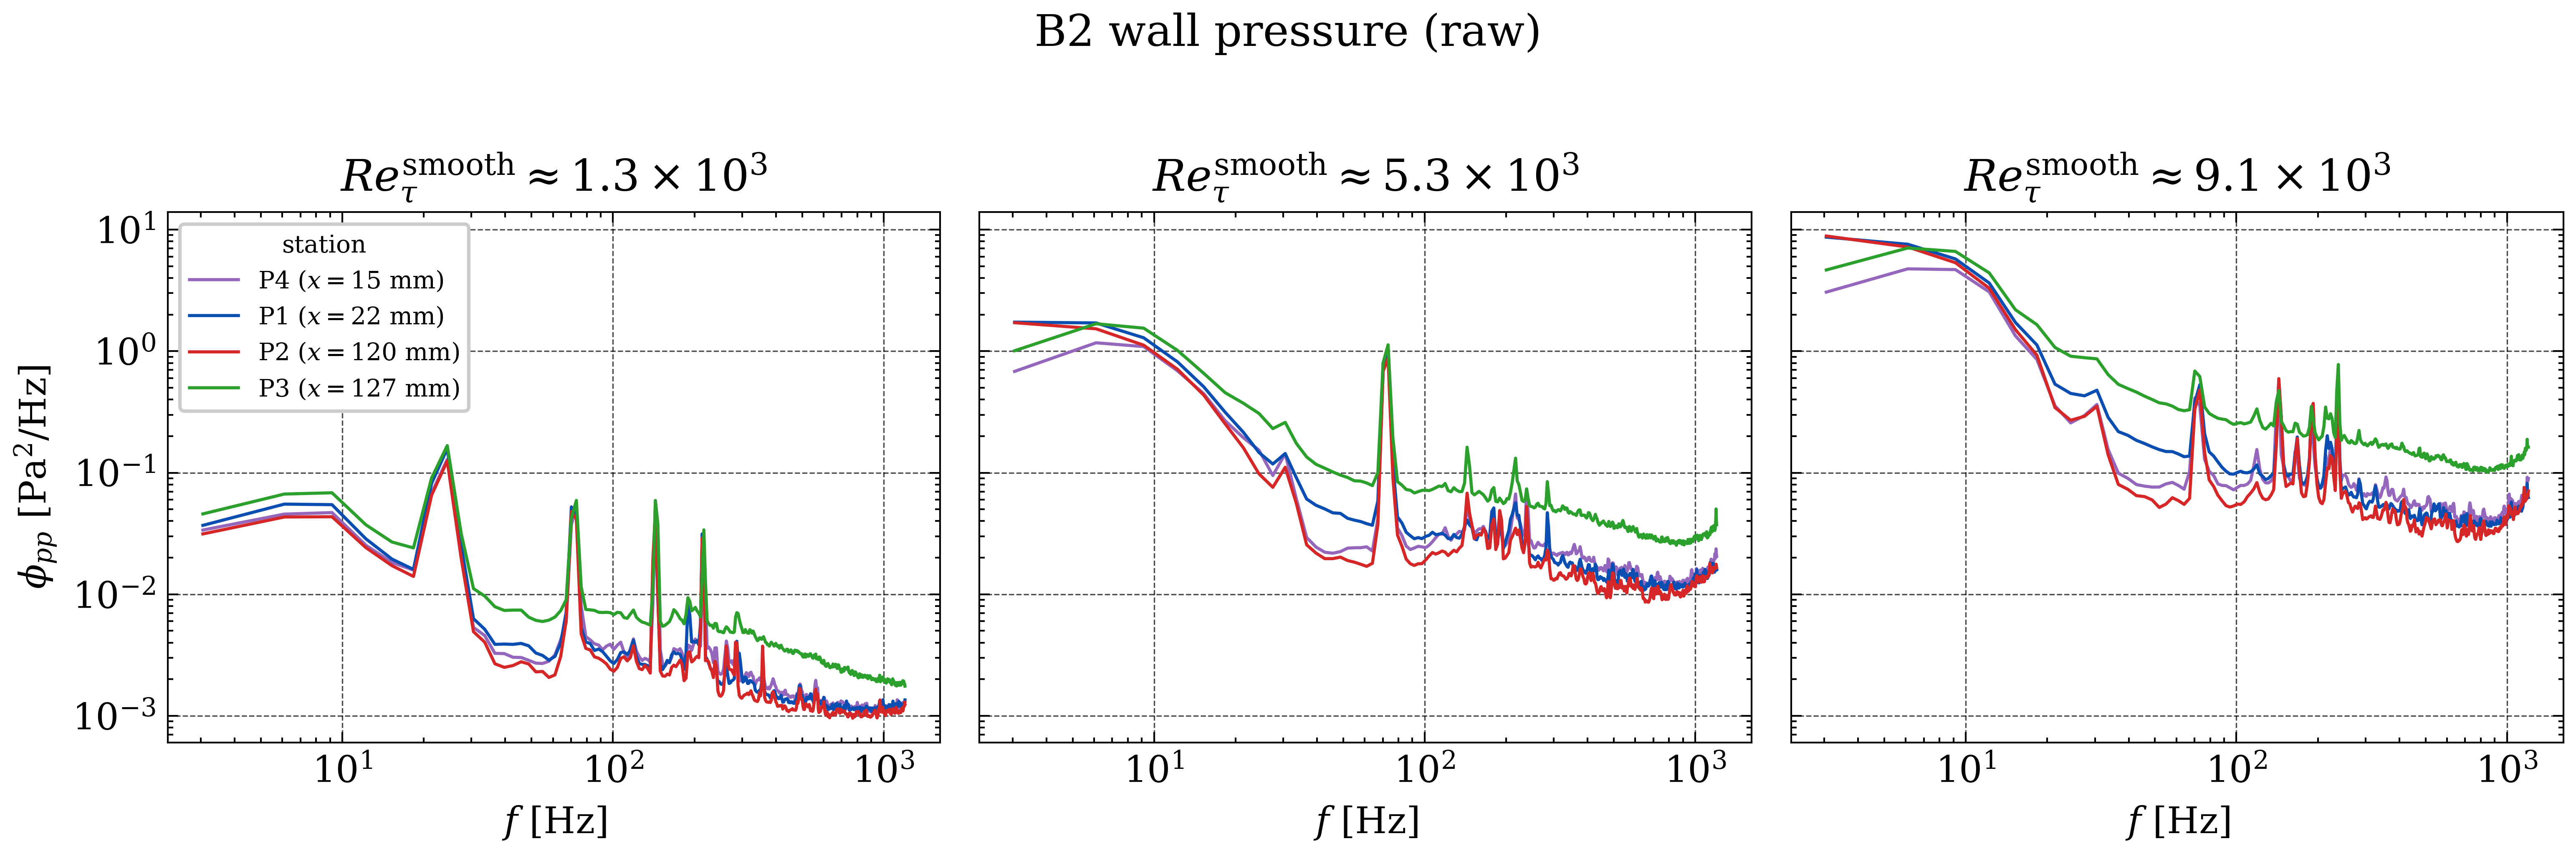
\includegraphics[width=\linewidth]{B2_wallp_raw}
    \caption{Raw wall-pressure PSD, $\phi_{pp}$ [Pa$^2$/Hz] against frequency, before facility-noise rejection (SU HPWT). One panel per pressurisation, labelled by $Re_\tau^{\mathrm{smooth}}$; all four pinhole stations per panel, each curve terminated at its per-station band edge $f_{\mathrm{cut}} \le 1.2$~kHz (below the pinhole Helmholtz resonance). Data: \texttt{E\_B2\_wallp\_SU\_raw.hdf5}.}
    \label{fig:wall pressure bump}
\end{figure}

Figure~\ref{fig:wall pressure bump} shows the wall-pressure spectra at the four stations with no facility-noise rejection applied, band-limited to the reported band.

\begin{figure}
    \centering
    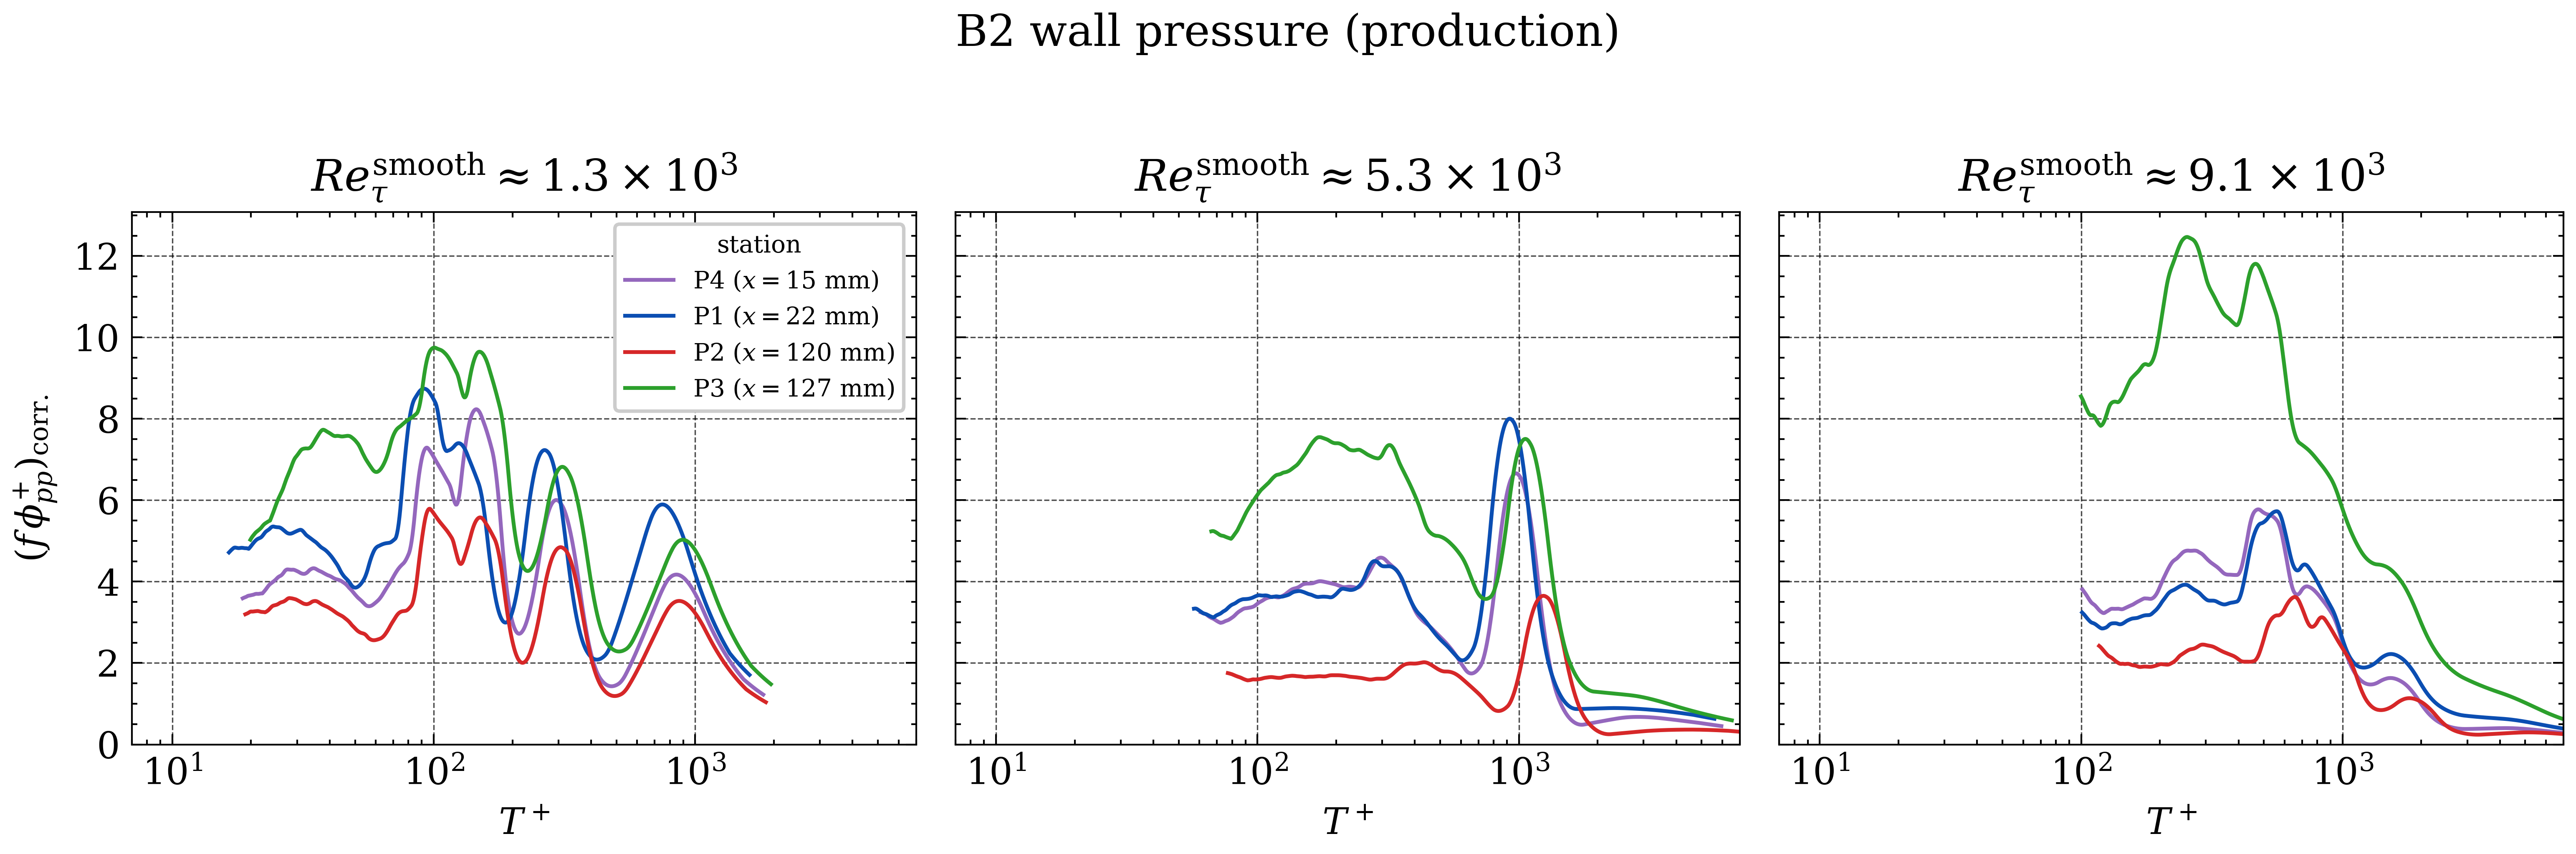
\includegraphics[width=\linewidth]{B2_wallp_production}
    \caption{Production (facility-noise-rejected via the smooth-wall-trained Wiener kernel), premultiplied, inner-scaled wall-pressure spectra (SU HPWT). One panel per pressurisation, labelled by $Re_\tau^{\mathrm{smooth}}$; all four stations per panel, each inner-scaled with its own measured $u_\tau$. The band edge $f_{\mathrm{cut}}$ sets the lowest $T^{+}$ shown. Data: \texttt{E\_B2\_wallp\_SU\_production.hdf5}.}
    \label{fig:wallp production bump}
\end{figure}

Figure~\ref{fig:wallp production bump} shows the bump wall pressure after the smooth-wall-trained Wiener rejection. In contrast to the fence, the rejection is essentially inert here: it changes the reported-band variance by at most $4\%$ (close stations at $0$~psig), ${\le}2\%$ at $50$~psig and a negligible amount elsewhere. This follows directly from the freestream anomaly above: the kernel subtracts the nose-cone signal scaled by the smooth-wall facility-to-wall transfer (order unity at the tones), but with the bump installed the wall-to-nose-cone tone ratio is $15$--$44$ times the smooth-wall value, so the subtracted noise estimate is over an order of magnitude too small to reach the facility content actually present at the wall. The B2 production signals are therefore, in practice, FRF-corrected and band-limited with only marginal facility-noise rejection, and the narrow spectral peaks that survive -- at $T^{+}\!\approx\!2.8\times10^{2}$ and ${\approx}8.5\times10^{2}$ at $0$~psig and $T^{+}\!\approx\!10^{3}$ at $50$~psig, the $70$ and ${\approx}23$~Hz facility tones -- are residual facility noise, not flow physics. The broad station-dependent structure, again largest at P3 and several times the smooth-wall baseline, is the genuine wall imprint of the bump-perturbed boundary layer, including its freestream-radiated sources, which the smooth-wall-trained rejection deliberately does not target.

\subsubsection{Wall pressure baseline verification}

\begin{figure}
    \centering
    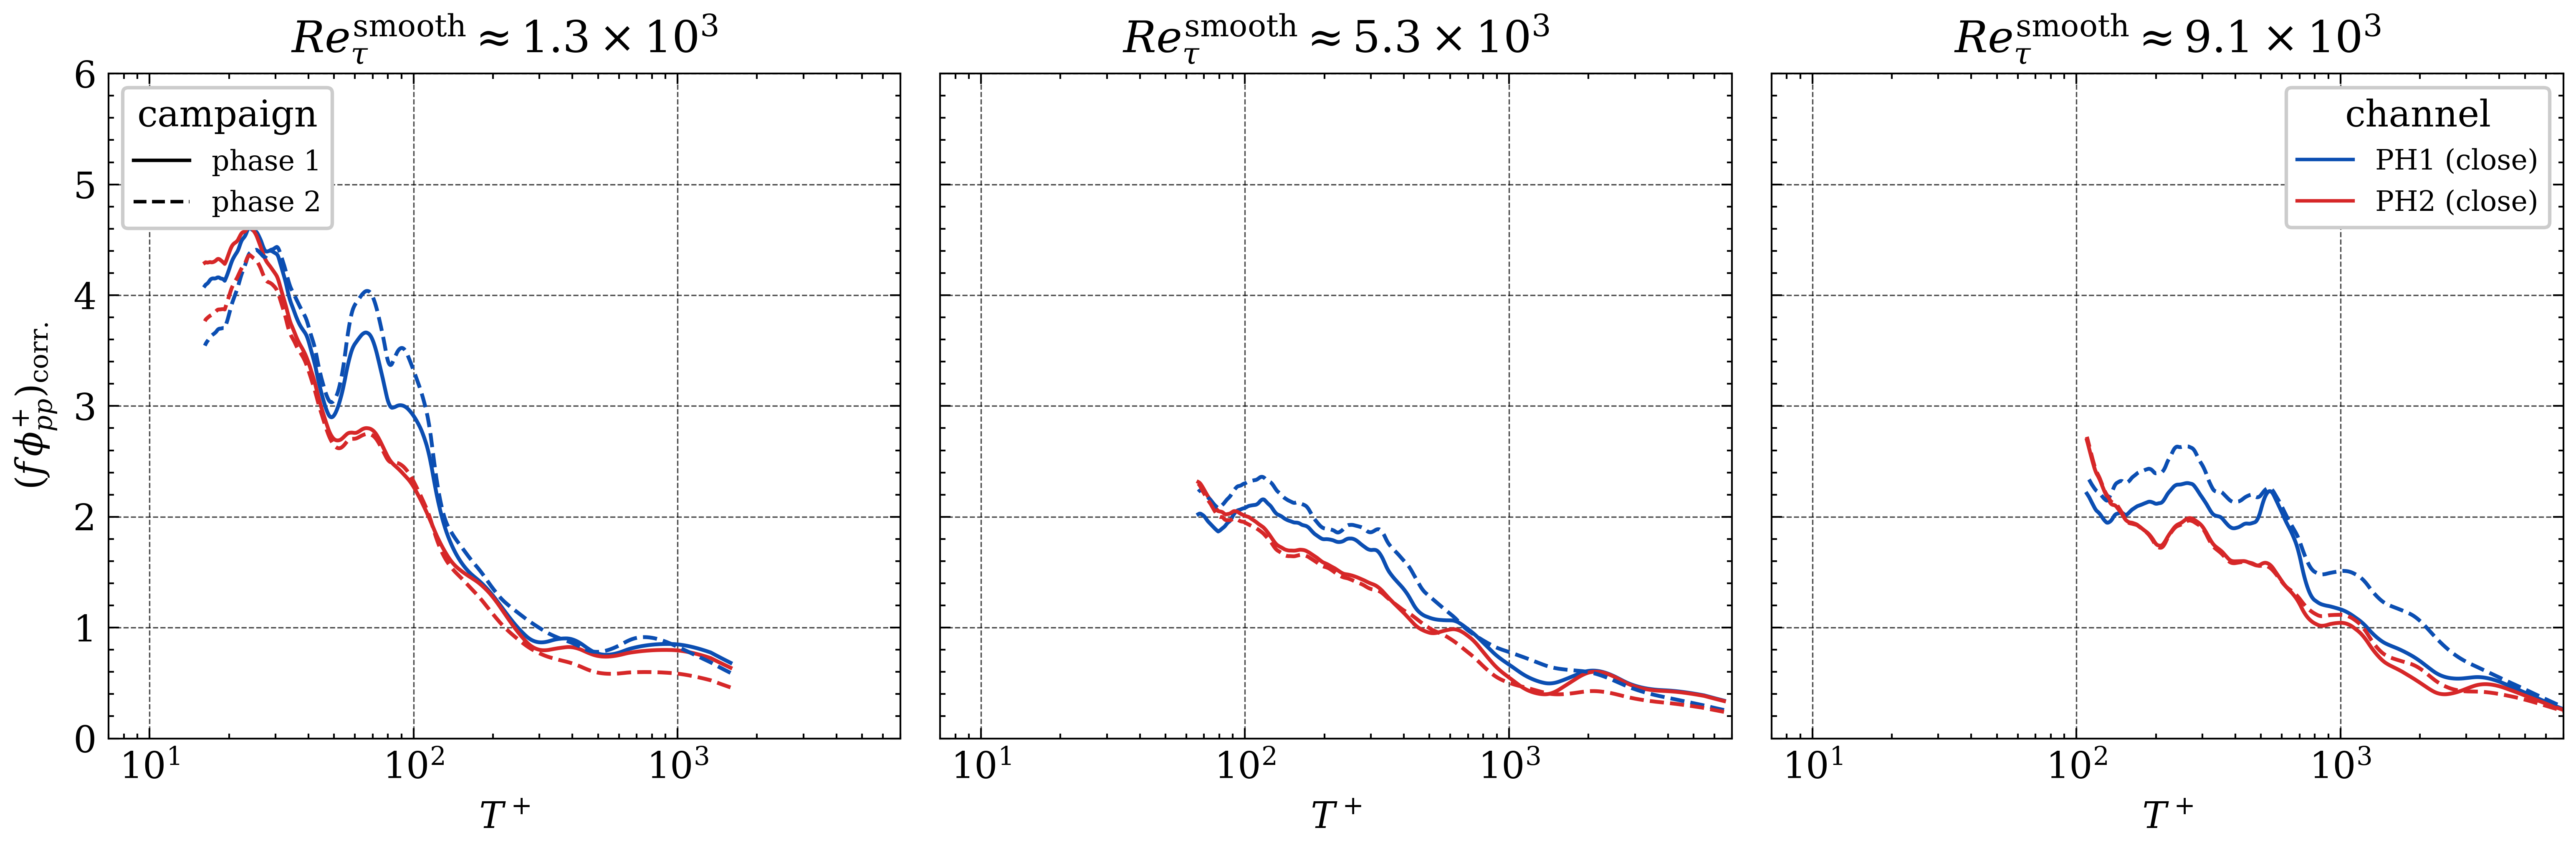
\includegraphics[width=\linewidth]{baseline_verification}
    \caption{Premultiplied, inner-normalised wall-pressure spectra of the smooth-wall baseline, one panel per pressurisation (labelled by $Re_\tau^{\mathrm{smooth}}$). Phase 1 (solid) and phase 2 (dashed), close-spacing PH1 (blue) and PH2 (red), band-limited at $f_{\mathrm{cut}}$. Shown is the baseline reported in phase 1 verified against identical measurements repeated after the phase-2 acquisition. Data: phase-1 and phase-2 smooth-wall baselines (\texttt{G\_wallp\_SU\_production.hdf5}); not part of the B1/B2 upload.}
    \label{fig:wall pressure SU verf}
\end{figure}

As a final check, we re-acquire the smooth-wall baseline of phase 1 after the bump and fence data are collected for phase 2. Figure~\ref{fig:wall pressure SU verf} overlays the phase-1 baseline and the post-phase-2 baseline on the same axes, both carried through the smooth-wall production pipeline: the same phase-1 pinhole calibration, and a Wiener rejection trained adaptively on each campaign's own smooth-wall records -- the correct procedure on a smooth wall, where the freestream reference carries facility noise only, and the same training that produces the fixed kernel transplanted to B1/B2. The two campaigns agree closely where the spectrum is turbulence-dominated: the premultiplied peak is reproduced to within ${\approx}10\%$ at every pressurisation, reported-band variances agree to within $16\%$ (phase-2/phase-1 ratios of $0.86$--$1.16$ over the six channel/condition combinations), and the median pointwise deviation of the smoothed inner-scaled spectra is $9$--$16\%$. Deviations exceeding ${\sim}30\%$ are confined to the lowest frequencies ($f \lesssim 140$~Hz, $T^{+} \gtrsim 7\times10^{2}$), where the incompletely rejected, run-to-run-variable facility contribution dominates. The smooth-wall reference is thus reproduced within the repeatability of the facility-noise environment over the full campaign, supporting the fidelity of the B1/B2 production data.

\vspace{2in}

\subsection{Case R1: Distributed sandgrain roughness}

\subsection{Case R2: Rough-to-smooth transition}
